% Requires in preamble:
% \usepackage{pgfplots}
% \pgfplotsset{compat=1.18}

\begin{figure}[htbp]
\centering
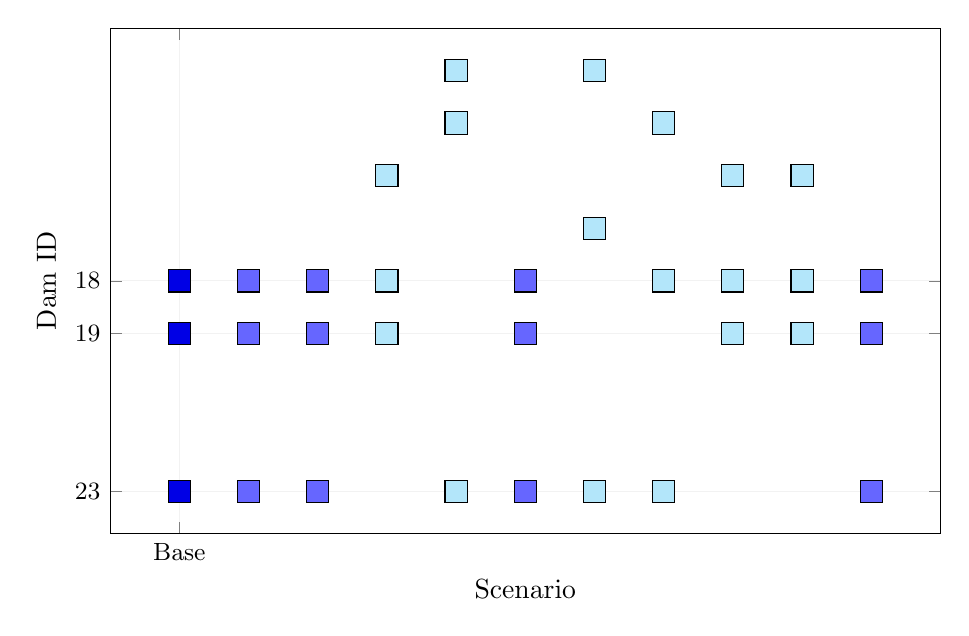
\begin{tikzpicture}
\begin{axis}[
  width=\textwidth,
  height=8cm,
  xlabel={Scenario},
  ylabel={Dam ID},
  xtick=data,
  ytick=data,
  symbolic x coords={Base,Test 1,Test 2,Test 3,Test 4,Test 5,Test 6,Test 7,Test 8,Test 9,Test 10},
  symbolic y coords={1,3,12,13,18,19,20,21,23},
  y dir=reverse,
  grid=both,
  grid style={opacity=0.2},
  tick label style={font=\small},
]
% Base (deep blue)
\addplot[
  only marks,
  mark=square*,
  mark size=4pt,
  draw=black,
  fill=blue!90!black
] coordinates {
  (Base,18) (Base,19) (Base,23)
};
% Matching Base selections in other scenarios (blue)
\addplot[
  only marks,
  mark=square*,
  mark size=4pt,
  draw=black,
  fill=blue!60
] coordinates {
  (Test 1,18) (Test 1,19) (Test 1,23)
  (Test 2,18) (Test 2,19) (Test 2,23)
  (Test 5,18) (Test 5,19) (Test 5,23)
  (Test 10,18) (Test 10,19) (Test 10,23)
};
% All other selections (light blue)
\addplot[
  only marks,
  mark=square*,
  mark size=4pt,
  draw=black,
  fill=cyan!30
] coordinates {
  (Test 3,12) (Test 3,18) (Test 3,19)
  (Test 4,1) (Test 4,3) (Test 4,23)
  (Test 6,1) (Test 6,13) (Test 6,23)
  (Test 7,3) (Test 7,18) (Test 7,23)
  (Test 8,12) (Test 8,18) (Test 8,19)
  (Test 9,12) (Test 9,18) (Test 9,19)
};
\end{axis}
\end{tikzpicture}
\caption{Scenario–dam selection map for the base WGP (first column) and ten test sets. Each filled square marks a selected dam site.}
\label{fig:weight_heatmap}
\end{figure}
